\section{Trajectory analysis} \label{ch:trajectory}

**intro**

\subsection{Governing equations}\label{sec:gov}

\begin{wrapfigure}{r}{0.4\textwidth}
		\centering
		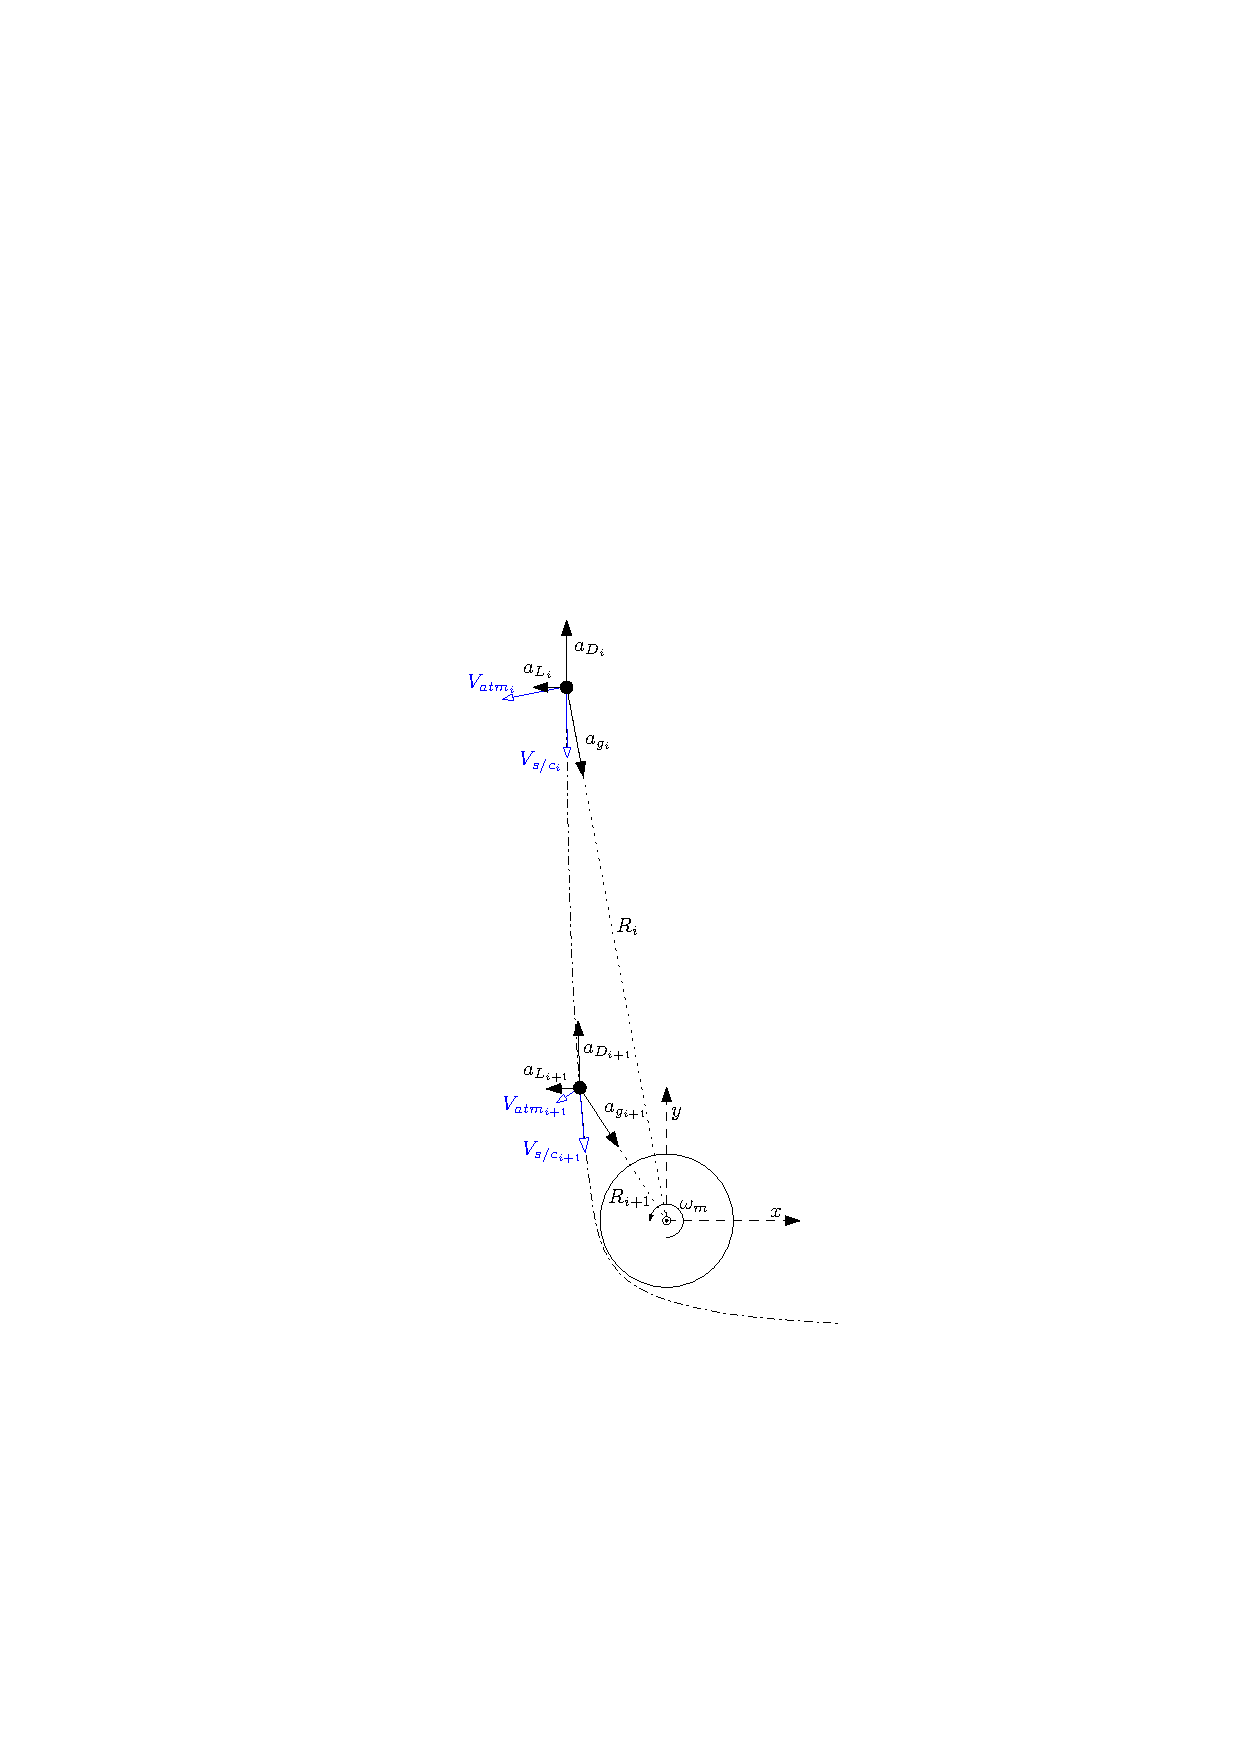
\includegraphics[width = 0.4\textwidth]{Figure/orbital_mechanics.pdf}
		\caption{The \gls{fbs} of the aeroshell mission}
		\label{fig:orb}
\end{wrapfigure}

The motion of a spacecraft can be broken down in some dominant contributors. These contributors are the gravitational pull and the aerodynamic forces. Disturbances like solar radiation or gravitational pull from moons or other bodies is neglected in the model.

The gravitational pull is described by Newtons law of gravitation


\subsection{Program structure}\label{sec:prog_struct}

In order to use the governing equations (equation \ref{eq:final}**!!need label!!**) to produce usefull results they have to be implemented in a simulation which calculates the trajectory. From this calculated trajectory the program has to extract usefull data and conclusions. Three different modules are discribed in subsection \ref{subsec:modules}. In subsection \ref{subsec:flow} a flowchart of the program is presented.

\subsection{Modules} \label{subsec:modules}

The program first implements the governing equations on each timestep. Secondly two modules were created, one to find feasible orbits and another to calculate the full orbit of the orbits which are found to be feasible. These three modules are described below.

\paragraph{Implementation of governing equations}

\paragraph{Orbit selection}

\paragraph{Full orbit simulation}

\subsection{Flowchart} \label{subsec:flow}
**flowchart

\begin{figure}[H]
\centering
\hspace{-23mm}
\includegraphics[width = 0.8\textwidth]{Figure/astro_tool.pdf}
\vspace{-5mm}
\caption{Flowchart of the working principle of the trajectory analysis program}
\label{fig:traj_flow}
\end{figure}

\subsection{Verification and validation}